% Options for packages loaded elsewhere
\PassOptionsToPackage{unicode}{hyperref}
\PassOptionsToPackage{hyphens}{url}
%
\documentclass[
  man,floatsintext]{apa6}
\usepackage{amsmath,amssymb}
\usepackage{lmodern}
\usepackage{iftex}
\ifPDFTeX
  \usepackage[T1]{fontenc}
  \usepackage[utf8]{inputenc}
  \usepackage{textcomp} % provide euro and other symbols
\else % if luatex or xetex
  \usepackage{unicode-math}
  \defaultfontfeatures{Scale=MatchLowercase}
  \defaultfontfeatures[\rmfamily]{Ligatures=TeX,Scale=1}
\fi
% Use upquote if available, for straight quotes in verbatim environments
\IfFileExists{upquote.sty}{\usepackage{upquote}}{}
\IfFileExists{microtype.sty}{% use microtype if available
  \usepackage[]{microtype}
  \UseMicrotypeSet[protrusion]{basicmath} % disable protrusion for tt fonts
}{}
\makeatletter
\@ifundefined{KOMAClassName}{% if non-KOMA class
  \IfFileExists{parskip.sty}{%
    \usepackage{parskip}
  }{% else
    \setlength{\parindent}{0pt}
    \setlength{\parskip}{6pt plus 2pt minus 1pt}}
}{% if KOMA class
  \KOMAoptions{parskip=half}}
\makeatother
\usepackage{xcolor}
\usepackage{graphicx}
\makeatletter
\def\maxwidth{\ifdim\Gin@nat@width>\linewidth\linewidth\else\Gin@nat@width\fi}
\def\maxheight{\ifdim\Gin@nat@height>\textheight\textheight\else\Gin@nat@height\fi}
\makeatother
% Scale images if necessary, so that they will not overflow the page
% margins by default, and it is still possible to overwrite the defaults
% using explicit options in \includegraphics[width, height, ...]{}
\setkeys{Gin}{width=\maxwidth,height=\maxheight,keepaspectratio}
% Set default figure placement to htbp
\makeatletter
\def\fps@figure{htbp}
\makeatother
\setlength{\emergencystretch}{3em} % prevent overfull lines
\providecommand{\tightlist}{%
  \setlength{\itemsep}{0pt}\setlength{\parskip}{0pt}}
\setcounter{secnumdepth}{-\maxdimen} % remove section numbering
% Make \paragraph and \subparagraph free-standing
\ifx\paragraph\undefined\else
  \let\oldparagraph\paragraph
  \renewcommand{\paragraph}[1]{\oldparagraph{#1}\mbox{}}
\fi
\ifx\subparagraph\undefined\else
  \let\oldsubparagraph\subparagraph
  \renewcommand{\subparagraph}[1]{\oldsubparagraph{#1}\mbox{}}
\fi
\newlength{\cslhangindent}
\setlength{\cslhangindent}{1.5em}
\newlength{\csllabelwidth}
\setlength{\csllabelwidth}{3em}
\newlength{\cslentryspacingunit} % times entry-spacing
\setlength{\cslentryspacingunit}{\parskip}
\newenvironment{CSLReferences}[2] % #1 hanging-ident, #2 entry spacing
 {% don't indent paragraphs
  \setlength{\parindent}{0pt}
  % turn on hanging indent if param 1 is 1
  \ifodd #1
  \let\oldpar\par
  \def\par{\hangindent=\cslhangindent\oldpar}
  \fi
  % set entry spacing
  \setlength{\parskip}{#2\cslentryspacingunit}
 }%
 {}
\usepackage{calc}
\newcommand{\CSLBlock}[1]{#1\hfill\break}
\newcommand{\CSLLeftMargin}[1]{\parbox[t]{\csllabelwidth}{#1}}
\newcommand{\CSLRightInline}[1]{\parbox[t]{\linewidth - \csllabelwidth}{#1}\break}
\newcommand{\CSLIndent}[1]{\hspace{\cslhangindent}#1}
\ifLuaTeX
\usepackage[bidi=basic]{babel}
\else
\usepackage[bidi=default]{babel}
\fi
\babelprovide[main,import]{english}
% get rid of language-specific shorthands (see #6817):
\let\LanguageShortHands\languageshorthands
\def\languageshorthands#1{}
% Manuscript styling
\usepackage{upgreek}
\captionsetup{font=singlespacing,justification=justified}

% Table formatting
\usepackage{longtable}
\usepackage{lscape}
% \usepackage[counterclockwise]{rotating}   % Landscape page setup for large tables
\usepackage{multirow}		% Table styling
\usepackage{tabularx}		% Control Column width
\usepackage[flushleft]{threeparttable}	% Allows for three part tables with a specified notes section
\usepackage{threeparttablex}            % Lets threeparttable work with longtable

% Create new environments so endfloat can handle them
% \newenvironment{ltable}
%   {\begin{landscape}\centering\begin{threeparttable}}
%   {\end{threeparttable}\end{landscape}}
\newenvironment{lltable}{\begin{landscape}\centering\begin{ThreePartTable}}{\end{ThreePartTable}\end{landscape}}

% Enables adjusting longtable caption width to table width
% Solution found at http://golatex.de/longtable-mit-caption-so-breit-wie-die-tabelle-t15767.html
\makeatletter
\newcommand\LastLTentrywidth{1em}
\newlength\longtablewidth
\setlength{\longtablewidth}{1in}
\newcommand{\getlongtablewidth}{\begingroup \ifcsname LT@\roman{LT@tables}\endcsname \global\longtablewidth=0pt \renewcommand{\LT@entry}[2]{\global\advance\longtablewidth by ##2\relax\gdef\LastLTentrywidth{##2}}\@nameuse{LT@\roman{LT@tables}} \fi \endgroup}

% \setlength{\parindent}{0.5in}
% \setlength{\parskip}{0pt plus 0pt minus 0pt}

% Overwrite redefinition of paragraph and subparagraph by the default LaTeX template
% See https://github.com/crsh/papaja/issues/292
\makeatletter
\renewcommand{\paragraph}{\@startsection{paragraph}{4}{\parindent}%
  {0\baselineskip \@plus 0.2ex \@minus 0.2ex}%
  {-1em}%
  {\normalfont\normalsize\bfseries\itshape\typesectitle}}

\renewcommand{\subparagraph}[1]{\@startsection{subparagraph}{5}{1em}%
  {0\baselineskip \@plus 0.2ex \@minus 0.2ex}%
  {-\z@\relax}%
  {\normalfont\normalsize\itshape\hspace{\parindent}{#1}\textit{\addperi}}{\relax}}
\makeatother

% \usepackage{etoolbox}
\makeatletter
\patchcmd{\HyOrg@maketitle}
  {\section{\normalfont\normalsize\abstractname}}
  {\section*{\normalfont\normalsize\abstractname}}
  {}{\typeout{Failed to patch abstract.}}
\patchcmd{\HyOrg@maketitle}
  {\section{\protect\normalfont{\@title}}}
  {\section*{\protect\normalfont{\@title}}}
  {}{\typeout{Failed to patch title.}}
\makeatother

\usepackage{xpatch}
\makeatletter
\xapptocmd\appendix
  {\xapptocmd\section
    {\addcontentsline{toc}{section}{\appendixname\ifoneappendix\else~\theappendix\fi\\: #1}}
    {}{\InnerPatchFailed}%
  }
{}{\PatchFailed}
\keywords{language acquisition; speech perception; infant-directed speech; adult-directed speech, test-retest reliability\newline\indent Word count: 4468}
\DeclareDelayedFloatFlavor{ThreePartTable}{table}
\DeclareDelayedFloatFlavor{lltable}{table}
\DeclareDelayedFloatFlavor*{longtable}{table}
\makeatletter
\renewcommand{\efloat@iwrite}[1]{\immediate\expandafter\protected@write\csname efloat@post#1\endcsname{}}
\makeatother
\usepackage{lineno}

\linenumbers
\usepackage{csquotes}
\ifLuaTeX
  \usepackage{selnolig}  % disable illegal ligatures
\fi
\IfFileExists{bookmark.sty}{\usepackage{bookmark}}{\usepackage{hyperref}}
\IfFileExists{xurl.sty}{\usepackage{xurl}}{} % add URL line breaks if available
\urlstyle{same} % disable monospaced font for URLs
\hypersetup{
  pdftitle={Assessing test-retest reliability of the infant preference measures},
  pdfauthor={Melanie S. Schreiner1,2 \& the ManyBabies Test-Retest Consortium},
  pdflang={en-EN},
  pdfkeywords={language acquisition; speech perception; infant-directed speech; adult-directed speech, test-retest reliability},
  hidelinks,
  pdfcreator={LaTeX via pandoc}}

\title{Assessing test-retest reliability of the infant preference measures}
\author{Melanie S. Schreiner\textsuperscript{1,2} \& the ManyBabies Test-Retest Consortium\textsuperscript{}}
\date{}


\shorttitle{test-retest reliability of the infant preference measures}

\authornote{

Correspondence concerning this article should be addressed to Melanie S. Schreiner, Gosslerstr. 14, 37073 Göttingen. E-mail: \href{mailto:melanie.schreiner@psych.uni-goettingen.de}{\nolinkurl{melanie.schreiner@psych.uni-goettingen.de}}

}

\affiliation{\vspace{0.5cm}\textsuperscript{1} University of Goettingen\\\textsuperscript{2} Leibniz Science Campus PrimateCognition}

\abstract{%
The ManyBabies1 collaborative research project (hereafter, MB1; Frank et al., 2017; ManyBabies Consortium, 2020) explores the reproducibility of the well-studied and robust phenomenon of infants' preference of infant-directed speech (hereafter, IDS) over adult-directed speech (hereafter, ADS; Cooper \& Aslin, 1990). The current study is a follow-on project aiming at further investigating the test-retest reliability of infant speech preference measures. In particular, labs of the original study were asked to bring in tested babies for a second appointment retesting infants on their IDS preference. This allows us to estimate test-retest reliability for the three different methods used to investigate preferential listening in infancy: The head-turn preference procedure, central fixation, and eye-tracking. Our results suggest that the test-retest reliability of infants' speech preference measures is rather low. While increasing the number of trials that infants needed to contribute for inclusion in the analysis from 2 to 8 trial pairs revealed a descriptive growth in test-retest reliability, it also considerably reduced the study's effective sample size. Therefore, future research on infant development should take into account that not all experimental measures might be appropriate to assess individual differences between infants, and hence, the interpretation of findings needs to be treated with caution.
}



\begin{document}
\maketitle

Obtaining a quantitative measure of young infant and children's cognitive abilities is an extraordinarily difficult endeavor; the most frequent way to assess what they know or can do is done via tracking overt behavior. However, the attention span of this specific group of participants is rather short, they do not follow instructions, their mood can change instantly and their behavior can be best described as unstable and volatile. Therefore, most measurements are noisy and the typical sample size of a study is often just around 20 infants per group resulting in low power (Oakes, 2017). In addition, there is individual and environmental variation that may add even more noise to the data (e.g., as discussed by Johnson \& Zamuner, 2010). Despite these demanding conditions, infancy researchers, nevertheless, need to have reliable and robust ways to assess infants' behavior.

In order to address these challenges in infant research, the ManyBabies collaborative research project was launched (Frank et al., 2017). Within a collaborative framework, the aim of this initiative is to conduct large-scale conceptual, consensus-based replications of seminal findings to identify sources of variability and establish best practices for experimental studies in infancy.

The fact that there is a substantial amount of literature on infants' preference of infant-directed speech (hereafter, IDS) over adult-directed speech (hereafter, ADS, Cooper \& Aslin, 1990) led to the decision of exploring the reproducibility of this well-studied phenomenon within the first ManyBabies collaborative research project (hereafter, MB1, ManyBabies Consortium, 2020). Across many different cultures, infants are commonly addressed in IDS, which typically is characterized by higher pitch, greater pitch range, and shorter utterances, compared to the language used between interacting adults (Fernald et al., 1989). A large body of behavioral studies finds that across ages and methods, infants show increased looking times when hearing IDS compared to ADS stimuli (Cooper \& Aslin, 1990; see Dunst, Gorman, \& Hamby, 2012 for a meta-analysis). This attentional enhancement is also documented in neurophysiological studies showing increased neural activation during IDS compared to ADS exposure (Naoi et al., 2012; Zangl \& Mills, 2007). In addition to the heightened attention, IDS has also been identified as facilitating early word learning. In particular, infants' word segmentation abilities Thiessen, Hill, \& Saffran (2005) and their learning of word-object associations (Graf Estes \& Hurley, 2013; Ma, Golinkoff, Houston, \& Hirsh-Pasek, 2011) seems to be enhanced in the context of IDS. In sum, IDS seems to be beneficial for early language development.

Within MB1, altogether 67 labs contributed data of 2,329 infants showing that babies generally prefer to listen to IDS over ADS. Nevertheless, the overall effect size \emph{d} = 0.35 was much smaller than the meta-analytic effect size of \emph{d} = 0.67 reported by Dunst et al. (2012). The results revealed a number of additional factors that influenced the effect size. First, there was a developmental change with older infants showing larger preferences. Second, the stimulus language was also linked to the speech preference with North American English learning infants being more likely to prefer IDS over ADS than infants learning other languages. Third, comparing the different methods employed, the head-turn preference procedure yielded the highest effect size, followed by the central fixation paradigm, with eye-tracking revealing the smallest effect size. Finally, exploratory analyses assessed the effect of different inclusion criteria. Across methods, using stricter inclusion criteria led to an increase in effect sizes despite the larger proportion of excluded participants (see also Byers-Heinlein, Bergmann, \& Savalei, 2021, for the relation between sample size, effect size, and exclusion criteria).

However, there is a difference between a result being reliable in a large sample of infants and the individual measure of an individual infant being reliable. In studies tracking individual differences, the measured behavior during an experimental setting is often used to predict a cognitive function or specific skill later in life. A precondition for this link to be observable is that inter-individual differences between infants do exist and can be detected with a high reliability at these earlier stages. However, how reliable are the measures used in infancy research?

A salient example of this line of individual differences research is the literature showing that infants' behavior in speech perception tasks can be linked to later language development (see Cristia, Seidl, Junge, Soderstrom, \& Hagoort, 2014 for a meta-analysis), potentially identifying infants at risk for later language delays or disorders. This finding thus has substantial implications for theoretical and applied work. However, to be able to make such claims robustly would require a high reliability within infants across multiple testing sessions. Previous attempts to address the reliability of measurements are either limited to adult populations investigating various tasks (Hedge, Powell, \& Sumner, 2018), or have been conducted with very small sample sizes (e.g., Houston, Horn, Qi, Ting, \& Gao, 2007).

In one example of such a study, Colombo, Mitchell, and Horowitz (1988) used a paired comparison task, in which infants were familiarized with a stimulus and for the test trials presented with the familiarized and a novel stimulus side-by-side. Results indicated that infants' novelty preference was extremely variable from task to task. Assessing infants' performance from one week to another revealed that infants' attention measures were moderately reliable. However, reliability seemed to increase with the number of tasks infants were able to complete in the younger age group suggesting that reliability is influenced by the number of assessments. In addition, infants' performance from 4 to 7 months was longitudinally stable but somewhat smaller than the week-to-week reliability.

Cristia, Seidl, Singh, and Houston (2016) also retested infant populations by independently conducting 12 different experiments on infant speech perception at three different labs with different implementations of the individual studies. Hence, it was only after completed data collection that the data was pooled together by the different labs revealing potential confounds. Nevertheless, the results showed that reliability was extremely variable across the different experiments and labs and overall low.

Against this background, the current study attempts to further explore test-retest reliability of infants' performance in an auditory preference task. Within MB1, a multilab collaboration, we examine whether infants' preferential listening behavior to IDS and ADS is reliable across two different test sessions. We also aim to address whether time between test and retest or infants' language background influences the reliability of the preference measure.

Our study was faced with a critical design choice: what stimulus to use to assess test-retest reliability. A first constraint of our study was that, since it was a follow-on to MB1, any stimulus we used would always be presented after the MB1 stimuli. One option would be simply to bring back infants and have them hear exactly the same stimulus materials. A weakness of this design would be the potential for stimulus familiarity effects, however, since infants would have heard the materials before. Further confusing matters, infants might show a preference for or against a familiar stimulus depending on their age (Hunter \& Ames, 1988). The ideal solution then would be to create a brand new stimulus set with the same characteristics. Unfortunately, because of the process of creating the MB1 stimuli, we did not have enough normed raw recordings available to make brand new stimulus items that conformed to the same standards as the MB1 stimuli.

Given this situation, we chose an intermediate path: we reversed the ordering of MB1 stimuli. Average looking times in MB1 were always lower than 9s per trial, even for the youngest children on the earliest trials (the group who looked the longest on average). So most children in MB1 did not hear the second half of most trials. Thus, by reversing the order, we had a perfectly matched stimulus set that was relatively unfamiliar to most infants. The disadvantage of this design was that infants who looked longer might be more likely to hear a familiar clip that they had heard in the previous study. If infants then showed a familiarity preference -- an assumption which might not be true -- the end result could be to inflate our estimates of test-retest reliability slightly, since longer lookers would on average look a bit longer at retest due to their familiarity preference. We view this risk as relatively low, but do note that it is a limitation of our design.\\
The MB1 study was also interested in effects of experimental method on infant-directed speech preference. Using central fixation (hereafter, CF), eye-tracking, and the head-turn preference procedure (hereafter, HPP), the current study also explores whether there are any differences in test-retest reliability between the three widely used methods. Exploring differences in CF, eye-tracking, and HPP, Junge et al. (2020) provide some evidence in favor of using the HPP in speech segmentation tasks. In addition, their re-analysis of the meta-analysis on infant speech segmentation conducted by Bergmann and Cristia (2016) also suggested numerically larger effect sizes for HPP than for eye-tracking. Similarly, the MB1 project reported an increase in the effect size for HPP compared to CF and eye-tracking (ManyBabies Consortium, 2020). HPP requires gross motor movements relative to other methods, such as CF and eye-tracking paradigms, for which subtle eye movements towards a monitor located in front of the child are sufficient. One possible explanation for the stronger effects with HPP may be a higher sensitivity to the contingency of the presentation of auditory stimuli and infants' head turns away from the typical forward-facing position. While these findings suggest that HPP may be a more sensitive index of infant preference, they do not translate into higher reliability for individual infants' performance using the different methods. Hence, it remains an open question whether the same measures that produce larger effect sizes at the group-level also have higher test-retest reliability for individual infants (Byers-Heinlein, Bergmann, et al., 2021). Therefore, assessing the test-retest reliability of the different preference measures is crucial, so that researchers can make informed decisions about the appropriate methods for their particular research question. Critically, only measures with high test-retest reliability should be used for studies of individual differences.

Preregistration. Prior to the start of data collection, we preregistered the current study on the Open Science Framework (OSF; see \url{https://osf.io/v5f8t}). We also had secondary planned analyses which were not run in the end as we had fewer participants than originally expected.

\hypertarget{method}{%
\section{Method}\label{method}}

A call was issued to all labs participating in the original MB1 study on January 24th, 2018 (ManyBabies Consortium, 2020). The collection of retest session data was initially set to end on May 31st, 2018, one month after the end date of the original MB1 project. Due to the fact that the original MB1 project extended the time frame for data collection and the late start of data collection for the MB1 test-retest study, we also allowed participating labs to continue data collection past the scheduled end date.

\hypertarget{participants}{%
\subsection{Participants}\label{participants}}

Contributing labs were asked to re-recruit their monolingual participants between the ages of 6 to 12 months who had already participated in the MB1 project. If participating labs had not committed to testing either of these age groups, they were also allowed to re-recruit participants from the youngest age group of 3- to 6-month-olds and/or the oldest age group of 12- to 15-month-olds. Labs were asked to contribute half (\emph{n}=16) or full sample (\emph{n}=32), however, a lab's data was included in the study regardless of the number of included infants. The study was approved by each lab's respective ethics committee and parental consent was obtained for each infant prior to participation in the study.

Our final sample consisted of 158 monolingual infants from 7 different labs. In order to be included in the study, infants needed a minimum of 90\% first language exposure, to be born full term with no known developmental disorders, and normal hearing and vision. We excluded 11 participants due to session errors and 11 participants who did not have at least one valid trial per condition (IDS and ADS) at their first or second session. The mean age of infants included in the study was 245 days (range: 108 -- 373 days). Further information on labs and participants are provided in Table 1.

\hypertarget{materials}{%
\subsection{Materials}\label{materials}}

\hypertarget{visual-stimuli.}{%
\subsubsection{Visual stimuli.}\label{visual-stimuli.}}

The visual stimuli were identical to MB1. For the central fixation paradigm and eye-tracking, labs were asked to use a multicolored static checkerboard as fixation stimulus as well as a multicolored moving circle with a ringing sound as an attention getter to reorient infants toward the screen in between trials. Labs using the HPP method were instructed to use their lab's standard procedure, as in MB1.

\hypertarget{speech-stimuli.}{%
\subsubsection{Speech stimuli.}\label{speech-stimuli.}}

We used the identical training stimuli of piano music from MB1. A second set of naturalistic IDS and ADS recordings of mothers either talking to their infant or to an experimenter was created for the retest session by reversing the order of clips within each sequence of the original study. This resulted in eight new sequences of natural IDS and eight new sequences of natural ADS with a length of 18 seconds each. This was in order to prevent infants who still remembered the stimuli from their first test session from easily getting bored.

\hypertarget{procedure.}{%
\subsubsection{Procedure.}\label{procedure.}}

Infants were retested using the identical procedure as during the first testing day: central fixation, HPP, or eye-tracking. Participating labs were asked to ideally schedule test and retest session 7 days apart with a minimum number of 1 day and a maximum number of 31 days. Three infants whose time between test and retest exceeded 31 days were also included in the analyses. The mean number of days between test and retest was 10 (range: 1 to 49 days).

A total of 18 trials, including two training, eight IDS, and eight ADS trials, were presented in one of four pseudo-randomized orders. Trial length was either infant-controlled or fixed depending on the lab's standard procedure, that is a trial stopped either if the infant looked away for 2 seconds or after the total trial duration of 18 seconds. The experimenter and the parent listened to music masked with the stimuli of the study via noise-cancelling headphones. If the experimenter was in an adjacent room, blinding was optional for the online coding experimenter.

\hypertarget{data-exclusion.}{%
\subsubsection{Data exclusion.}\label{data-exclusion.}}

A child was excluded if they had a session error, i.e., an experimenter error (e.g., inaccurate coding, or presentation of retest stimuli on the first test session), or equipment failure (visual stimuli continued to play after the end of a trial). Trials were excluded if they were marked as trial error, i.e., infant was reported to be fussy, incorrect use of stimuli, or parental interference, or if the minimum looking time of 2 s was not met. If a participant was unable to contribute at least one IDS and one ADS trial for either test or retest, all data of that participant was excluded from the test-retest analyses.

\hypertarget{results}{%
\section{Results}\label{results}}

\begin{table}[tbp]

\begin{center}
\begin{threeparttable}

\caption{\label{tab:labs}Statistics of the included labs. n refers to the number of infants included in the final analysis.}

\begin{tabular}{lllll}
\toprule
Lab & \multicolumn{1}{c}{Method} & \multicolumn{1}{c}{Language} & \multicolumn{1}{c}{Mean age (days)} & \multicolumn{1}{c}{N}\\
\midrule
babylab-potsdam & HPP & German & 227 & 22\\
babyling-oslo & Eyetracking & Norwegian & 249 & 10\\
brookes-babylab & central fixation & English & 267 & 18\\
InfantCog-UBC & central fixation & English & 147 & 7\\
infantll-madison & HPP & English & 230 & 30\\
lancslab & Eyetracking & English & 236 & 16\\
wsi-goettingen & central fixation & German & 280 & 39\\
wsi-goettingen & HPP & German & 242 & 16\\
\bottomrule
\end{tabular}

\end{threeparttable}
\end{center}

\end{table}

\hypertarget{ids-preference}{%
\subsection{IDS preference}\label{ids-preference}}

First, we examined infants' preferences for IDS in both sessions. Two two-samples t-tests revealed that the children in Session 1, \(t(157) = 6.16\), \(p < .001\), and in Session 2, \(t(157) = 4.55\), \(p < .001\), showed a preference of IDS over ADS (see Table 2 for the looking times in each session). In the first session, 67.09 percent of the children showed a preference for IDS, and in the second session, 63.92 percent of the children showed a numerical preference for IDS. In other words, we replicated the previous finding from the main MB1 study. There was no difference in the strength of the preference effect, as a multilevel analysis with a random slope and random intercept for session on the lab level revealed no significant impact of session on infants' preference, with an estimate of zero and very small variance, \(\beta\)=-0.01, \emph{SE}=0.04, \emph{p}=.756.

\begin{table}[tbp]

\begin{center}
\begin{threeparttable}

\caption{\label{tab:descriptives_table1}Looking times in s for each session and condition}

\begin{tabular}{lllll}
\toprule
Trial type & Session 1 $Mean$ & Session 1 $SD$ & Session 2 $Mean$ & Session 2 $SD$\\
\midrule
ADS & 7.72 & 2.77 & 6.96 & 2.92\\
IDS & 8.76 & 2.85 & 7.75 & 2.75\\
\bottomrule
\end{tabular}

\end{threeparttable}
\end{center}

\end{table}

\hypertarget{reliability}{%
\subsection{Reliability}\label{reliability}}

\begin{table}[tbp]

\begin{center}
\begin{threeparttable}

\caption{\label{tab:coef_table2}Coefficient estimates from a linear mixed effects model predicting IDS preference in Session 2.}

\begin{tabular}{lllll}
\toprule
 & \multicolumn{1}{c}{Estimate} & \multicolumn{1}{c}{SE} & \multicolumn{1}{c}{t} & \multicolumn{1}{c}{p}\\
\midrule
Intercept & 0.143 & 0.070 & 2.050 & 0.086\\
Session One & -0.060 & 0.089 & -0.677 & 0.499\\
\bottomrule
\end{tabular}

\end{threeparttable}
\end{center}

\end{table}

We assessed test-retest reliability in two ways. First, we conducted a multilevel analysis, with Lab as random intercept, predicting the IDS preference in Session 2 based on the IDS preference in Session 1. The results revealed that we could not predict the preference score in Session 2 based on Session 1 (see Table 2). Second, we calculated the Pearson correlation coefficient. While a simple correlation coefficient might overestimate the test-retest reliability in our sample because it does not control for the differences between different labs and methods (HPP, CF, and eye-tracking), we felt it was important to also conduct a Pearson correlation as it is commonly used to assess reliability. Again, the size of the correlation coefficient was not statistically different from zero and the estimate was, in fact, approaching nil, \(r = .03\), 95\% CI \([-.12, .19]\), \(t(156) = 0.43\), \(p = .670\). Furthermore, we calculated the percentage of preference reversal between test and retest counting the number of participants for whom the preference changed between test and retest, and dividing it by the number of all participants. The results revealed that 46.20 percent of the infants had a preference reversal from test to retest session. Taken together, our results lead us to conclude that there is no overall test-retest reliability for the three infant preference measures used within the current study.

To test whether the results were different for a specific method, we calculated the Pearson correlation coefficients and the multilevel analyses for the three different methods, HPP, central fixation and eye-tracking, separately (see Table 4). Splitting the data per method also did not lead to different results. Neither the Pearson correlation coefficients nor the coefficients of the multilevel analysis were significant, all \emph{p}-values \textgreater{} .286.
We also tested for the possibility that the Time between sessions might have an impact on the reliability. The subsequent multilevel analysis, with Lab as random intercept, predicting the IDS preference in Session 2 based on the IDS preference in Session 1, the number of days between Session 1 and Session 2 and the interaction of these two variables, did not indicate that Time between sessions had an effect. Neither the main effect of Time between sessions, \(\beta\)=0.00, \emph{SE}=0, \emph{p}=.740, nor the interaction term, \(\beta\)=-0.02, \emph{SE}=0.02, \emph{p}=.277, showed significant effects.
As NAE-learning infants showed greater IDS preferences than their non-NAE counterparts in the original study, we also assessed if test-retest reliability interacted with children's native language. A multilevel analysis with Lab as random intercept, predicting the IDS preference in Session 2 based on the IDS preference in Session 1, NAE and the interaction of these two variables, revealed no interaction, \(\beta\)=0.24, \emph{SE}=0.19, \emph{p}=.214 (see Figure 1).

\begin{table}[tbp]

\begin{center}
\begin{threeparttable}

\caption{\label{tab:unnamed-chunk-6}Coefficient estimates from a linear mixed effects model predicting IDS preference in Session 2 for each method separately.}

\begin{tabular}{llllll}
\toprule
Method & \multicolumn{1}{c}{estimate} & \multicolumn{1}{c}{SE} & \multicolumn{1}{c}{pvalue} & \multicolumn{1}{c}{cor} & \multicolumn{1}{c}{pvalue2}\\
\midrule
HPP & 0.005 & 0.138 & 0.968 & 0.005 & 0.968\\
Eyetracking & -0.190 & 0.238 & 0.432 & -0.161 & 0.432\\
central fixation & -0.197 & 0.132 & 0.142 & 0.120 & 0.345\\
\bottomrule
\end{tabular}

\end{threeparttable}
\end{center}

\end{table}

\begin{figure}
\centering
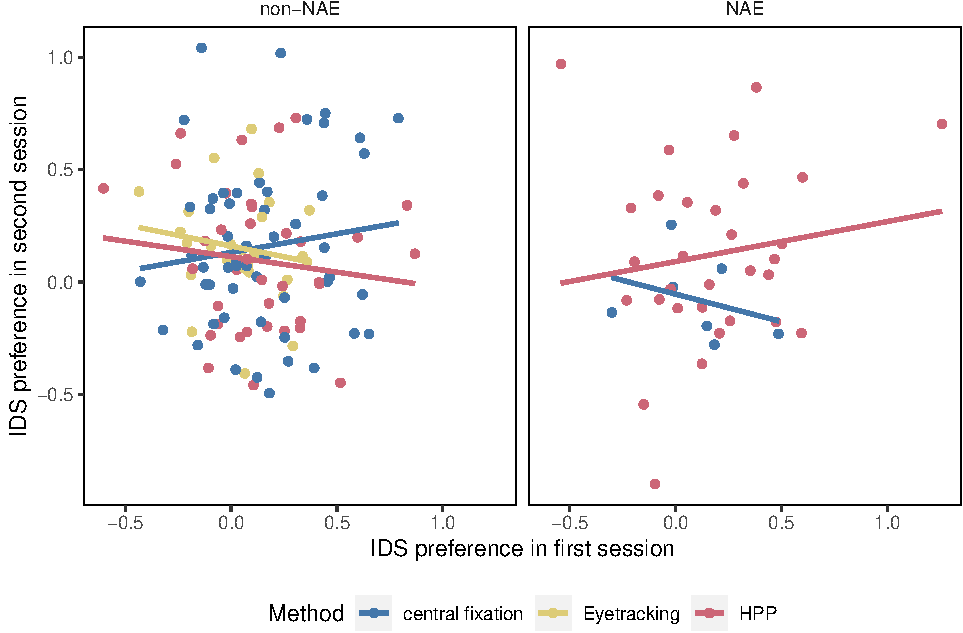
\includegraphics{Retest_current_draft_files/figure-latex/fig1-1.pdf}
\caption{\label{fig:fig1}Infants' preference in Session 1 and Session 2 with individual data points and regression lines color-coded by method (central fixation, eye-tracking, or HPP). Results are plotted separately for North American English-learning infants (right panel) and infants learning other languages and dialects (right panel).}
\end{figure}

\hypertarget{results-with-different-inclusion-criteria}{%
\subsection{Results with different inclusion criteria}\label{results-with-different-inclusion-criteria}}

To this point, all analyses were performed on data with the inclusion criteria from MB1. For this, infants needed only 1 out of 8 valid trial pairs (i.e., any combination of an IDS and ADS trial) to be included in the analyses. Given that the use of more stringent inclusion criteria yielded larger effects sizes within the original MB1 study, we also assessed test-retest reliability by applying stricter inclusion criteria and thereby increasing test length to 2, 4, 6, and 8 included test trial pairs per condition. Applying a stricter criterion - and thereby increasing test length - increased reliability numerically from r = .02 to r = .38 (Figure 2). However, in part likely due to the decrease in sample size, none of these correlations was statistically significant: 2 valid trial pairs, \(t(152) = 0.27\), \(p = .789\); 4 valid trial pairs, \(t(143) = 0.51\), \(p = .611\); 6 valid trial pairs, \(t(98) = 1.90\), \(p = .061\); 8 valid trial pairs - all trials on both testing days - \(t(22) = 1.93\), \(p = .067\). Nevertheless, the analyses show that stricter inclusion criteria might lead to higher test-retest reliability but at the same time comes with tremendous decreases in sample size.

\begin{figure}

{\centering 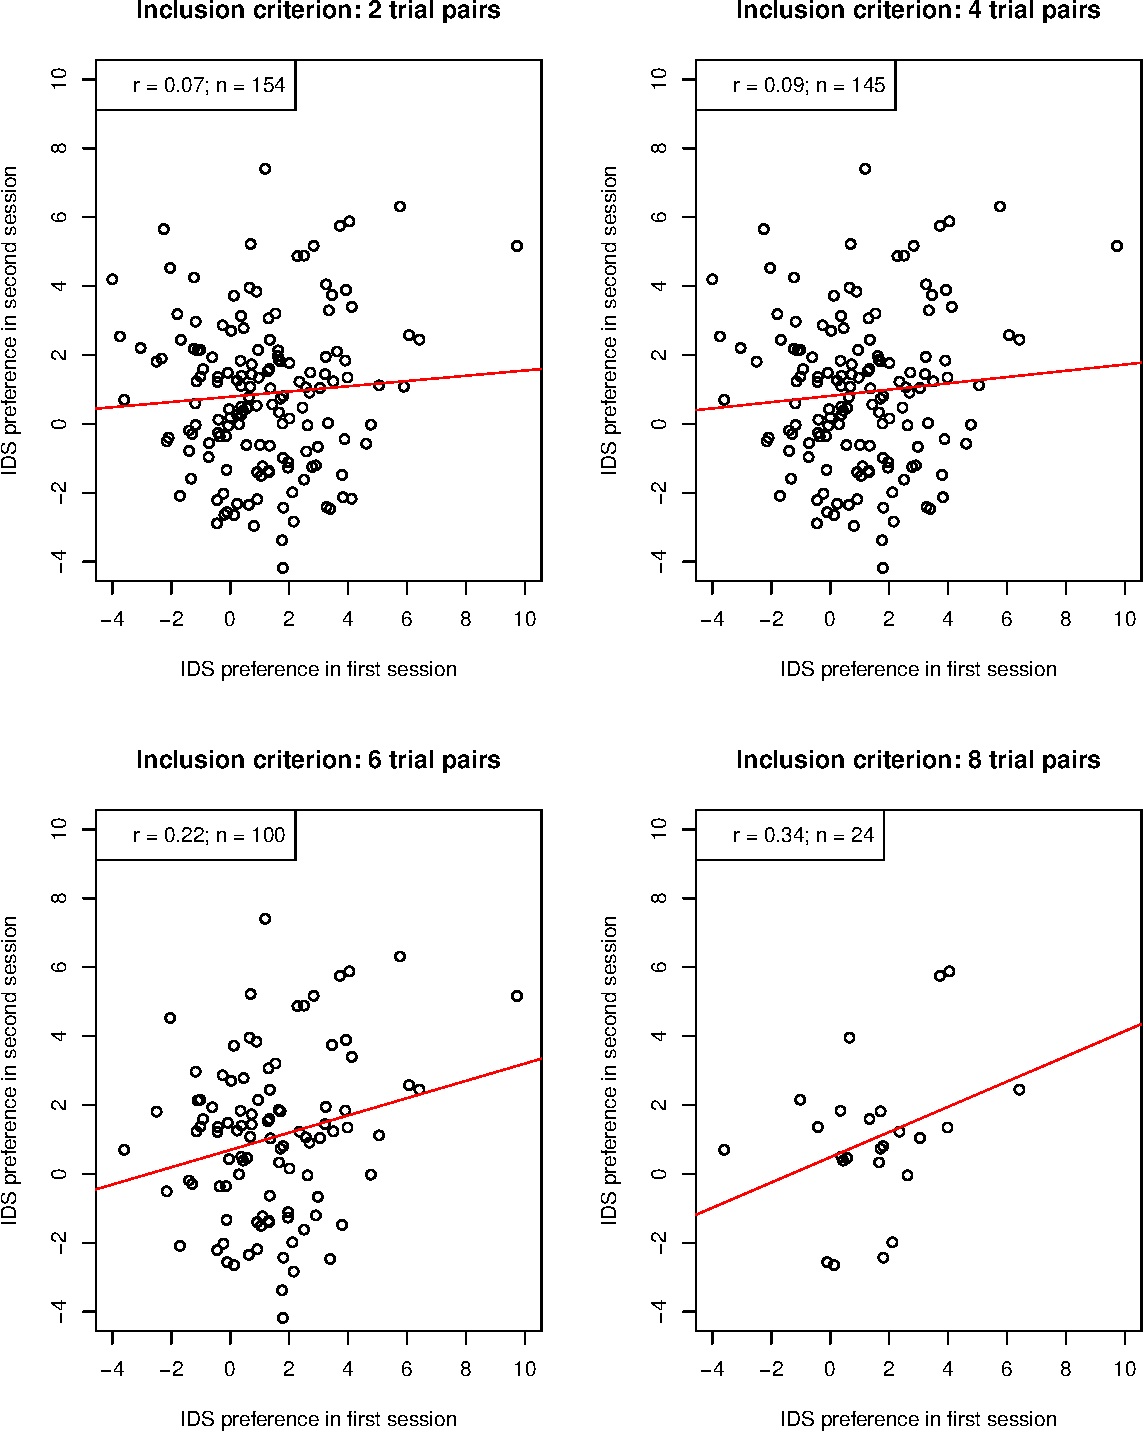
\includegraphics[width=5in]{Retest_current_draft_files/figure-latex/unnamed-chunk-8-1} 

}

\caption{IDS preferences of both sessions plotted against each other for each inclusion criterion. n indicates the number of included infants, r is the Pearson correlation coefficient as the indicator for reliability.}\label{fig:unnamed-chunk-8}
\end{figure}

\hypertarget{general-discussion}{%
\section{General Discussion}\label{general-discussion}}

The current study set out to explore the test-retest reliability of the infant speech preference of IDS over ADS. Infants of the original MB1 project were retested on a reversed order of stimuli in order to assess if their listening pattern would be similar to that of their initial assessment. While we replicated the original effect of infants' speech preference for IDS over ADS in the current MB1 follow-up study for both test and retest session on the group-level using the same MB1 protocol, we found that infants' speech preference measures had no test-retest reliability. In other words, we were unable to detect any stable individual differences of infants' speech preference. This finding is in line with other research indicating a rather low test-reliability for different developmental paradigms (Cristia et al., 2016). Given that most experimental procedures conducted in developmental research are interested in the comparison of groups, individual differences between participants within a specific condition are usually minimized by the experimental procedure while differences between conditions are maximized. Therefore, the infant preference measure may be a good approach to capture universal phenomena but does not seem to be appropriate for examining factors that may lead to individual differences in development.

Consistent with general psychometric theory (e.g., DeBolt, Rhemtulla, \& Oakes, 2020) a larger number of included test trials was associated with higher reliability. However, in our dataset, this association was based on exploratory analyses and was only found descriptively, hence, a replication is warranted. A similar effect on the group-level was found in the MB1 project, where a stricter inclusion criterion led to bigger effect sizes (ManyBabies Consortium, 2020).

In our study, as in the MB1 original study, higher reliability through strict exclusions came at a high cost. In particular, with the strictest criterion, only a small portion of the original sample size, that is 24 out of 158 infants, could be included in the final sample for this particular analysis. In other words, applying a stricter criterion leads to a higher drop out rate and reduces the actual sample size enormously. In the case of studies in the field of developmental science, where there are many practical restrictions in collecting large samples of infants (e.g., birth rate in the area, restricted lab capacities, budget restrictions), a strict drop out criterion might not be easy - if even possible at all - to implement. Note that studies in developmental science already have above average drop out rates (Miller, 2017). In addition, drop out may not be random, and so having high drop out rates can further limit the generalisability of a study. Particularly in the context of turning individual differences measures into diagnostic tools, high drop-out rates have an additional limitation of not being broadly usable.

An alternative approach to increase the number of valid trials might be to also increase the number of collected trials. In this case, a participant can have a high number/proportion of invalid trials and still be included into the final sample as the absolute number of trials is high and thereby decreasing trial-to-trial variability (DeBolt et al., 2020; see Silverstein, Feng, Westermann, Parise, \& Twomey, 2021 for an example). While this approach might sound promising, it must be seen if this is realistic, because the attention span of a typical participant of a developmental study is rather short. Therefore, prolonging the experimental procedure to maximize the absolute number of trials might also be practically challenging. Further potential attempts in obtaining higher numbers of valid trials may include changes in the procedure (e.g., Egger, Rowland, \& Bergmann, 2020) or implementing multi-day test sessions (Fernald \& Marchman, 2012).
As our results are only based on the particular phenomenon of IDS preference (albeit, with three widely used methods: HPP, central fixation; eye-tracking) it is essential to further assess the underlying reliability of these measures within other areas of speech perception. While most infants prefer IDS over ADS (Dunst et al., 2012), predicting a pattern of preference, for instance, within speech segmentation tasks, i.e.~familiar versus novel words, seem not that straightforward (Bergmann \& Cristia, 2016). Especially in the context of relating a direction of preference to later language development, there seem to be controversial findings. That is, both familiarity and novelty responses have been suggested to be predictive of infants' later linguistic abilities (DePaolis, Vihman, \& Keren-Portnoy, 2014; R. S. Newman, Rowe, \& Ratner, 2016; R. Newman, Ratner, Jusczyk, Jusczyk, \& Dow, 2006). In light of findings from the current study, researchers conducting longitudinal studies with experimental data from young infants predicting future outcomes should be cautious as there may be inter-individual variability affecting their preferences.

\hypertarget{limitations}{%
\subsection{Limitations}\label{limitations}}

While we had an above average sample size for a study in developmental research, we were unable to reach the number of participants collected within the original MB1 study. In addition to a delayed call, the extra effort of having to schedule a second lab visit for each participant and the fact that there were already other collaborative studies taking place simultaneously (MB1B, Byers-Heinlein, Tsui, Bergmann, et al., 2021; MB1G, Byers-Heinlein, Tsui, Van Renswoude, et al., 2021), might have contributed to the rather low turnout. A higher sample size and a larger number of participating labs from different countries might have enabled us to test for possible differences of the test-retest reliability of the different methods (HPP, central fixation, eye-tracking) and NAE versus non-NAE language backgrounds. Further, a larger sample size might have enabled us to conduct meaningful tests of moderators such as age of the child on the test-retest reliability.

A further limitation concerns the stimuli. While the order of the clips within trials presented to the participating children in the second session was different than in the first session, the exact same stimulus material as in MB1 was used in both sessions. In particular, all children heard the exact same voices in Session 1 and in Session 2. From a practical point of view, it was the easiest solution. However, familiarity effects might have influenced infants' looking behavior. Assuming that only infants with longer looking times in Session 1 might have had the chance to recognize the voices in Session 2 from their session a week ago as familiar clips would only be towards the end of trials, infants with shorter looking times might not have had the opportunity to listen to the voices from their first session. Therefore, for some children, familiarity with the stimulus material might have led to artificially lowering test-retest reliability.

\hypertarget{conclusion}{%
\section{Conclusion}\label{conclusion}}

Following the MB1 protocol, the current study could not detect test-retest reliability of infants' preference measures for IDS over ADS. Subsequent analyses showed that a stricter criterion for the inclusion of data points may enhance the test-retest reliability at the cost of high drop out rates. Developmental studies which rely on stable individual differences of their participants need to consider the underlying reliability of their measures, and we recommend a broader assessment of test-retest reliability in infant research.

\newpage

\hypertarget{data-and-materials-availability-statement}{%
\section{Data and materials availability statement}\label{data-and-materials-availability-statement}}

The data and materials that support the findings of the current study are openly available on OSF at \url{https://osf.io/ZEQKA/}.

\newpage

\hypertarget{references}{%
\section{References}\label{references}}

\begingroup
\setlength{\parindent}{-0.5in}
\setlength{\leftskip}{0.5in}

\hypertarget{refs}{}
\begin{CSLReferences}{1}{0}
\leavevmode\vadjust pre{\hypertarget{ref-bergmann2016development}{}}%
Bergmann, C., \& Cristia, A. (2016). Development of infants' segmentation of words from native speech: A meta-analytic approach. \emph{Developmental Science}, \emph{19}(6), 901--917.

\leavevmode\vadjust pre{\hypertarget{ref-byers2021six}{}}%
Byers-Heinlein, K., Bergmann, C., \& Savalei, V. (2021). Six solutions for more reliable infant research. \emph{Infant and Child Development}, e2296.

\leavevmode\vadjust pre{\hypertarget{ref-byers2021multilab}{}}%
Byers-Heinlein, K., Tsui, A. S. M., Bergmann, C., Black, A. K., Brown, A., Carbajal, M. J., et al.others. (2021). A multilab study of bilingual infants: Exploring the preference for infant-directed speech. \emph{Advances in Methods and Practices in Psychological Science}, \emph{4}(1), 2515245920974622.

\leavevmode\vadjust pre{\hypertarget{ref-byers2021development}{}}%
Byers-Heinlein, K., Tsui, R. K.-Y., Van Renswoude, D., Black, A. K., Barr, R., Brown, A., et al.others. (2021). The development of gaze following in monolingual and bilingual infants: A multi-laboratory study. \emph{Infancy}, \emph{26}(1), 4--38.

\leavevmode\vadjust pre{\hypertarget{ref-colombo1988infant}{}}%
Colombo, J., Mitchell, D. W., \& Horowitz, F. D. (1988). Infant visual attention in the paired-comparison paradigm: Test-retest and attention-performance relations. \emph{Child Development}, 1198--1210.

\leavevmode\vadjust pre{\hypertarget{ref-cooper1990preference}{}}%
Cooper, R. P., \& Aslin, R. N. (1990). Preference for infant-directed speech in the first month after birth. \emph{Child Development}, \emph{61}(5), 1584--1595.

\leavevmode\vadjust pre{\hypertarget{ref-cristia2014predicting}{}}%
Cristia, A., Seidl, A., Junge, C., Soderstrom, M., \& Hagoort, P. (2014). Predicting individual variation in language from infant speech perception measures. \emph{Child Development}, \emph{85}(4), 1330--1345.

\leavevmode\vadjust pre{\hypertarget{ref-cristia2016test}{}}%
Cristia, A., Seidl, A., Singh, L., \& Houston, D. (2016). Test--retest reliability in infant speech perception tasks. \emph{Infancy}, \emph{21}(5), 648--667.

\leavevmode\vadjust pre{\hypertarget{ref-debolt2020robust}{}}%
DeBolt, M. C., Rhemtulla, M., \& Oakes, L. M. (2020). Robust data and power in infant research: A case study of the effect of number of infants and number of trials in visual preference procedures. \emph{Infancy}, \emph{25}(4), 393--419.

\leavevmode\vadjust pre{\hypertarget{ref-depaolis2014infants}{}}%
DePaolis, R. A., Vihman, M. M., \& Keren-Portnoy, T. (2014). When do infants begin recognizing familiar words in sentences? \emph{Journal of Child Language}, \emph{41}(1), 226--239.

\leavevmode\vadjust pre{\hypertarget{ref-dunst2012preference}{}}%
Dunst, C., Gorman, E., \& Hamby, D. (2012). Preference for infant-directed speech in preverbal young children. \emph{Center for Early Literacy Learning}, \emph{5}(1), 1--13. Retrieved from \url{http://www.earlyliteracylearning.org/cellreviews/cellreviews_v5_n1.pdf}

\leavevmode\vadjust pre{\hypertarget{ref-egger2020improving}{}}%
Egger, J., Rowland, C. F., \& Bergmann, C. (2020). Improving the robustness of infant lexical processing speed measures. \emph{Behavior Research Methods}, \emph{52}(5), 2188--2201.

\leavevmode\vadjust pre{\hypertarget{ref-fernald2012individual}{}}%
Fernald, A., \& Marchman, V. A. (2012). Individual differences in lexical processing at 18 months predict vocabulary growth in typically developing and late-talking toddlers. \emph{Child Development}, \emph{83}(1), 203--222.

\leavevmode\vadjust pre{\hypertarget{ref-fernald1989cross}{}}%
Fernald, A., Taeschner, T., Dunn, J., Papousek, M., Boysson-Bardies, B. de, \& Fukui, I. (1989). A cross-language study of prosodic modifications in mothers' and fathers' speech to preverbal infants. \emph{Journal of Child Language}, \emph{16}(3), 477--501.

\leavevmode\vadjust pre{\hypertarget{ref-floccia2016british}{}}%
Floccia, C., Keren-Portnoy, T., DePaolis, R., Duffy, H., Delle Luche, C., Durrant, S., \ldots{} Vihman, M. (2016). British english infants segment words only with exaggerated infant-directed speech stimuli. \emph{Cognition}, \emph{148}, 1--9.

\leavevmode\vadjust pre{\hypertarget{ref-frank2017collaborative}{}}%
Frank, M. C., Bergelson, E., Bergmann, C., Cristia, A., Floccia, C., Gervain, J., \ldots{} Yurovsky, D. (2017). A collaborative approach to infant research: Promoting reproducibility, best practices, and theory-building. \emph{Infancy}, \emph{22}(4), 421--435. \url{https://doi.org/10.1111/infa.12182}

\leavevmode\vadjust pre{\hypertarget{ref-graf2013infant}{}}%
Graf Estes, K., \& Hurley, K. (2013). Infant-directed prosody helps infants map sounds to meanings. \emph{Infancy}, \emph{18}(5), 797--824. \url{https://doi.org/10.1111/infa.12006}

\leavevmode\vadjust pre{\hypertarget{ref-hedge2018reliability}{}}%
Hedge, C., Powell, G., \& Sumner, P. (2018). The reliability paradox: Why robust cognitive tasks do not produce reliable individual differences. \emph{Behavior Research Methods}, \emph{50}(3), 1166--1186.

\leavevmode\vadjust pre{\hypertarget{ref-houston2007assessing}{}}%
Houston, D. M., Horn, D. L., Qi, R., Ting, J. Y., \& Gao, S. (2007). Assessing speech discrimination in individual infants. \emph{Infancy}, \emph{12}(2), 119--145.

\leavevmode\vadjust pre{\hypertarget{ref-hunter1988multifactor}{}}%
Hunter, M. A., \& Ames, E. W. (1988). A multifactor model of infant preferences for novel and familiar stimuli. \emph{Advances in Infancy Research}, \emph{5}, 69--95.

\leavevmode\vadjust pre{\hypertarget{ref-johnson2010using}{}}%
Johnson, E., \& Zamuner, T. (2010). \emph{Using infant and toddler testing methods in language acquisition research.}

\leavevmode\vadjust pre{\hypertarget{ref-junge2020contrasting}{}}%
Junge, C., Everaert, E., Porto, L., Fikkert, P., Klerk, M. de, Keij, B., \& Benders, T. (2020). Contrasting behavioral looking procedures: A case study on infant speech segmentation. \emph{Infant Behavior and Development}, \emph{60}, 101448.

\leavevmode\vadjust pre{\hypertarget{ref-ma2011word}{}}%
Ma, W., Golinkoff, R. M., Houston, D. M., \& Hirsh-Pasek, K. (2011). Word learning in infant-and adult-directed speech. \emph{Language Learning and Development}, \emph{7}(3), 185--201.

\leavevmode\vadjust pre{\hypertarget{ref-manybabies2020quantifying}{}}%
ManyBabies Consortium. (2020). Quantifying sources of variability in infancy research using the infant-directed-speech preference. \emph{Advances in Methods and Practices in Psychological Science}, \emph{3}(1), 24--52.

\leavevmode\vadjust pre{\hypertarget{ref-miller2017developmental}{}}%
Miller, S. A. (2017). \emph{Developmental research methods}. Sage publications.

\leavevmode\vadjust pre{\hypertarget{ref-naoi2012cerebral}{}}%
Naoi, N., Minagawa-Kawai, Y., Kobayashi, A., Takeuchi, K., Nakamura, K., Yamamoto, J., \& Shozo, K. (2012). Cerebral responses to infant-directed speech and the effect of talker familiarity. \emph{Neuroimage}, \emph{59}(2), 1735--1744.

\leavevmode\vadjust pre{\hypertarget{ref-newman2016input}{}}%
Newman, R. S., Rowe, M. L., \& Ratner, N. B. (2016). Input and uptake at 7 months predicts toddler vocabulary: The role of child-directed speech and infant processing skills in language development. \emph{Journal of Child Language}, \emph{43}(5), 1158--1173.

\leavevmode\vadjust pre{\hypertarget{ref-newman2006infants}{}}%
Newman, R., Ratner, N. B., Jusczyk, A. M., Jusczyk, P. W., \& Dow, K. A. (2006). Infants' early ability to segment the conversational speech signal predicts later language development: A retrospective analysis. \emph{Developmental Psychology}, \emph{42}(4), 643.

\leavevmode\vadjust pre{\hypertarget{ref-oakes2017sample}{}}%
Oakes, L. M. (2017). Sample size, statistical power, and false conclusions in infant looking-time research. \emph{Infancy}, \emph{22}(4), 436--469.

\leavevmode\vadjust pre{\hypertarget{ref-schreiner2017listen}{}}%
Schreiner, M. S., \& Mani, N. (2017). Listen up! Developmental differences in the impact of IDS on speech segmentation. \emph{Cognition}, \emph{160}, 98--102.

\leavevmode\vadjust pre{\hypertarget{ref-silverstein2021infants}{}}%
Silverstein, P., Feng, J., Westermann, G., Parise, E., \& Twomey, K. E. (2021). Infants learn to follow gaze in stages: Evidence confirming a robotic prediction. \emph{Open Mind}, 1--15.

\leavevmode\vadjust pre{\hypertarget{ref-singh2009influences}{}}%
Singh, L., Nestor, S., Parikh, C., \& Yull, A. (2009). Influences of infant-directed speech on early word recognition. \emph{Infancy}, \emph{14}(6), 654--666.

\leavevmode\vadjust pre{\hypertarget{ref-thiessen2005infant}{}}%
Thiessen, E. D., Hill, E. A., \& Saffran, J. R. (2005). Infant-directed speech facilitates word segmentation. \emph{Infancy}, \emph{7}(1), 53--71. \url{https://doi.org/10.1207/s15327078in0701_5}

\leavevmode\vadjust pre{\hypertarget{ref-zangl2007increased}{}}%
Zangl, R., \& Mills, D. L. (2007). Increased brain activity to infant-directed speech in 6-and 13-month-old infants. \emph{Infancy}, \emph{11}(1), 31--62. \url{https://doi.org/10.1207/s15327078in1101_2}

\end{CSLReferences}

\endgroup


\end{document}
